\documentclass[a4paper]{article}
\usepackage{graphicx}
\usepackage{float}
\author{Hein van Beers \qquad Student number: 0765658 \\{\tt h.a.v.beers@student.tue.nl}\\ \\ Jeroen van Hoof \qquad Student number: 0778486 \\{\tt j.m.a.p.v.hoof@student.tue.nl}}
\title{Automated Reasoning\\
	 \large Practical assignment, Part I}
\begin{document}
	\maketitle
	
	\section*{Problem 1: Delivery for magic factory}
	Satisfying all constraints, find the maximum number of pallets of prittles that can be delivered, and show how for that number all pallets may be divided over the six trucks.

	
	\subsection*{Solution:}
	We generalize this problem to $n$ trucks. For each pallet place in a truck we introduce five variables, one for each type of building block. We have eight pallet places per truck, so we introduce $8*5*n = 40*n$ variables $p_{ijk}$ for $i = 1,\ldots,n$, $j = 1,\ldots,8$ and $k = 1,\ldots,5$ where for every $i,j,k$ the value of $p_{ijk}$ will be true if and only if a pallet of building block type $k$ will be put on pallet position $j$ in truck $i$.
	
	As the weight of each of the $n$ trucks may not exceed the capacity of 7800 kg, we express this by the formula
\[ \bigwedge_{i=1}^n (\sum_{k=1}^5 (\sum_{j=1}^8 (f(p_{ijk})*w_k)) \leq 7800).\]
Where $f(p_{ijk}) = 1$ if $p_{ijk}$ is equal to true and 0 otherwise. Also $w_k$ is the weight of a pallet of type $k$. In the table below you can see the weights of the different types of pallets.

\begin{table}[H]
\centering
\caption{Weights of the different types of pallets}
\label{my-label}
\begin{tabular}{c|c|c}
\textbf{Pallet type} & \textbf{Corresponding k} & \textbf{Weight (kg)} \\ \hline
Nuzzles              & 1                        & 700                  \\ \hline
Prittles             & 2                        & 800                  \\ \hline
Skipples             & 3                        & 1000                 \\ \hline
Crottles             & 4                        & 1500                 \\ \hline
Dupples              & 5                        & 100                 
\end{tabular}
\end{table}

	As prittles and crottles are not allowed to be put in the same truck, that is, for every two distinct positions $j,m$ in truck $i$ it is not allowed that both $p_{ij2}$ and $p_{im4}$ are true. This is expressed by the formula
\[ \bigwedge_{i=1}^n (\neg (\bigvee_{j=1}^8 p_{ij2}) \vee \neg (\bigvee_{m=1}^8 p_{im4})).\]

Next we assume that the first two trucks are cooled, so pallets of skipples cannot be placed in trucks 3 upto and including $n$. We express this by the formula
\[ \bigwedge_{i=3}^n \bigwedge_{j=1}^8 \neg p_{ij3}.\]

No two pallets of the type dupples may be placed in the same truck, that is, for every two distinct positions $j,m$ in truck $i$ it is not allowed that both $p_{ij5}$ and $p_{im5}$ are true. This is expressed by the formula
\[ \bigwedge_{i=1}^n \bigwedge_{j,m:1 \leq j < m \leq 8} \neg p_{ij5} \vee \neg p_{im5}.\]

Similarly, we also need the requirement that at most one variable is set to true per pallet position in a truck. So for every two distinct pallet types $k,m$ on position $j$ in truck $i$ it is not allowed that both $p_{ijk}$ and $p_{ijm}$ are true. This is expressed by the formula
\[ \bigwedge_{i=1}^n \bigwedge_{j=1}^8 \bigwedge_{k,m:1 \leq k < m \leq 5} \neg p_{ijk} \vee \neg p_{ijm}.\]

Finally, we consider the requirements of the demands. As the amount of pallets that need to be delivered for each pallet type is given, except for the prittles, we can express this by the formula
\[ \bigwedge_{k=1}^5 ( \sum_{i=1}^n ( \sum_{j=1}^8 f(p_{ijk}) ) = a_k).\]
Where $f(p_{ijk}) = 1$ if $p_{ijk}$ is equal to true and 0 otherwise. And $a_k$ is the amount of a pallets of type $k$ that need to be delivered. In the table below you can see the amount for each type of pallet.

\begin{table}[H]
\centering
\caption{Demand of each type of pallets}
\label{my-label}
\begin{tabular}{c|c|c}
\textbf{Pallet type} & \textbf{Corresponding k} & \textbf{Demand (pallets)} \\ \hline
Nuzzles              & 1                        & 4                  		\\ \hline
Prittles             & 2                        & ?                  		\\ \hline
Skipples             & 3                        & 8                 		\\ \hline
Crottles             & 4                        & 10                 		\\ \hline
Dupples              & 5                        & 5                 
\end{tabular}
\end{table}

For getting the answer to the maximization problem, we just try different values for the amount of pallets of prittles that need to be delivered and see if we get a solution. When we find a solution for a value $x$ for the amount of prittles that we deliver and we cannot find a solution for value $x+1$, we know that $x$ is the maximum number of pallets of prittles that can be delivered.\\

After trying several values, we found that 18 pallets of prittles is the maximum amount we can deliver, since the program does not yield a solution for 19 pallets of prittles.\\

The total formula now consists of the conjunction of all these ingredients, that is,
\[ \bigwedge_{i=1}^n (\sum_{k=1}^5 (\sum_{j=1}^8 (p_{ijk}*w_k)) \leq 7800) \;\; \wedge \]
\[ \bigwedge_{i=1}^n (\neg (\bigvee_{j=1}^8 p_{ij2}) \vee \neg (\bigvee_{m=1}^8 p_{im4})) \;\; \wedge \]
\[ \bigwedge_{i=3}^n \bigwedge_{j=1}^8 (\neg p_{ij3}) \;\; \wedge \]
\[ \bigwedge_{i=1}^n \bigwedge_{j,m:1 \leq j < m \leq 8} (\neg p_{ij5} \vee \neg p_{im5}) \;\; \wedge \]
\[ \bigwedge_{i=1}^n \bigwedge_{j=1}^8 \bigwedge_{k,m:1 \leq k < m \leq 5} (\neg p_{ijk} \vee \neg p_{ijm}) \;\; \wedge \]
\[ \bigwedge_{k=1}^5 ( \sum_{i=1}^n ( \sum_{j=1}^8 p_{ijk} ) = a_k) \]


This formula is easily expressed in SMT syntax, for instance, for $n=6$ one can generate

{\footnotesize

{\tt (benchmark Assignment1.smt}

{\tt :logic QF\_LIA}

{\tt :extrapreds (}

{\tt ;Truck 1 }

{\tt (p111) (p112) (p113) (p114) (p115) }

{\tt (p121) (p122) (p123) (p124) (p125) }

{\tt (p131) (p132) (p133) (p134) (p135) }

{\tt (p141) (p142) (p143) (p144) (p145) }

{\tt (p151) (p152) (p153) (p154) (p155) }

{\tt (p161) (p162) (p163) (p164) (p165) }

{\tt (p171) (p172) (p173) (p174) (p175) }

{\tt (p181) (p182) (p183) (p184) (p185) }

{\tt ;Truck 2 }

{\tt (p211) (p212) (p213) (p214) (p215) }

{\tt (p221) (p222) (p223) (p224) (p225) }

$\cdots \cdots$

{\tt )}

{\tt :formula}

{\tt   (and}

{\tt (<= (+ }

{\tt (* (ite p111 1 0) 700) $\cdots$ (* (ite p181 1 0) 700)}

{\tt (* (ite p112 1 0) 800) $\cdots$ (* (ite p182 1 0) 800)}

$\cdots \cdots$

{\tt (* (ite p115 1 0) 100) $\cdots$ (* (ite p185 1 0) 100)}

{\tt ) 7800)}

$\cdots \cdots$

{\tt (or }

{\tt (not (or p112 p122 p132 p142 p152 p162 p172 p182)) }

{\tt (not (or p114 p124 p134 p144 p154 p164 p174 p184)) }

{\tt ) }

$\cdots \cdots$

{\tt )) }
}

Applying {\tt yices -m -smt Assignment1.smt} yields the following result
within a fraction of a second:

{\footnotesize

{\tt sat }

{\tt (= p185 false)}

{\tt (= p445 false)}

{\tt (= p213 true)}

{\tt (= p214 false)}

{\tt (= p452 false)}

{\tt (= p233 true)}

{\tt (= p435 false)}

{\tt (= p474 true)}

{\tt (= p623 false)}

{\tt (= p531 true)}

{\tt (= p662 false)}

$\cdots \cdots$ }

The values that are are true for each truck are 
\[p113, p125, p134, p143, p153, p163, p173, p183 \]
\[p213, p222, p233, p242, p255, p262, p272, p282 \]
\[p312, p322, p332, p342, p352, p362, p372, p382 \]
\[p414, p424, p444, p464, p474, p485 \]
\[p512, p525, p531, p541, p552, p562, p572, p582 \]
\[p611, p621, p634, p644, p665, p674, p684 \]
Expressed in a picture this yields

\begin{figure}[H]
			\centering
				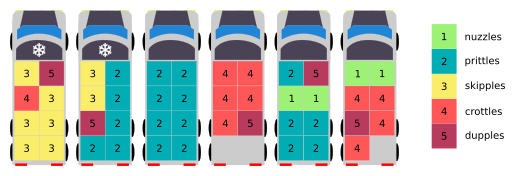
\includegraphics[scale=1]{trucks-2.png}
			\caption{Placement of pallets on truck. The first two trucks have facility for cooling skipples.}
		\end{figure}

We check that indeed all requirements are satisfied and we also see that the amount of pallets of prittles we can deliver is 18, since the program does not yield a solution for 19 pallets of prittles.\\

{\bf Remark:}
After doing exercise 2 of this assignment, we discovered that we could also use integers for the amount pallets of each type of building block per truck. In that way we would not need to determine each pallet place exactly, but only restrict the amount of pallets per truck to not exceed the maximum amount of pallets per truck. We would then only need one variable for each pallet type for each truck, which is $5*6=35$ variables. This is much less than the amount of variables we have now, so this implementation would greatly decrease the size of our requirements and increase the efficiency of our program. However, the solution will still be the same and since we did not have sufficient time to redo/rewrite the whole first exercise, we have chosen to not implement it in this way. But keep it in mind for future exercises and leave it here as an improvement.\\

{\bf Generalization:} 
As we generalized our approach for $n$ trucks rather than 6, it is interesting to see what happens for other values of $n$. For $n > 10$ we can still represent clearly what truck, pallet position and pallet type we want to indicate, since the pallet position cannot take on a value higher than eight and the pallet type cannot take on a value higher than 5. So if we keep the notation then it is still clear that {\tt p1111} represents truck 11, pallet position 1 and pallet type 1, which is nuzzles.

	\section*{Problem 2: Placing components on a power grid}
	To identify each component, we have named them $a, b, ... h$, with sizes $9 \times 7$, $12 \times 6$, $10 \times 7$, $18 \times 5$, $20 \times 4$, $10 \times 6$, $8 \times 6$ and $10 \times 8$. Furthermore, we named the power components $i, j, k$. 
	The specification that each component can be turned to $90^{\circ}$, can be simplified to swapping the x and y dimensions of a component with each other. For each component, we introduce predicates $a\_turned, b\_turned, ..., k\_turned$ to indicate rotation, and $a\_lx, a\_ly, b\_lx, b\_ly, ..., k\_lx, k\_ly,$ for the lengths and widths of $a, b, ..., k$. So the dimensions of each component are determined as follows:

	{\tt (= a\_lx (ite a\_turned 7 9))}
	
	{\tt (= a\_ly (ite a\_turned 9 7))}
	
	{\tt ...}
	
	\noindent We identify the origin of each component, with predicates $a\_ox, a\_oy, b\_ox, b\_oy, ..., k\_ox, k\_oy$ to denote x-origins and y-origins. To specify the size of the chip, we have to make sure that all components are within the limits of the length and width:
	
	{\tt (<= (+ a\_lx a\_ox) 29)}
	
	{\tt (>= a\_ox 0)}
	
	{\tt (<= (+ a\_ly a\_oy) 22)}
	
	{\tt (>= a\_oy 0)}
	
	{\tt ...}
	
	\noindent We must also make sure that none of the components overlap. To make sure that two components, a and b, do not overlap, one of four statements must hold:
	\begin{itemize}
		\item \textbf{b} is right of \textbf{a} $\Leftrightarrow a\_ox >= b\_x + b\_lx$
		\item \textbf{b} is left of \textbf{a} $\Leftrightarrow b\_ox >= a\_ox + a_lx$
		\item \textbf{b} is below \textbf{a} $\Leftrightarrow a\_oy >= b\_oy + b\_ly$
		\item \textbf{b} is above \textbf{a} $\Leftrightarrow b\_oy >= a\_oy + a\_ly$
	\end{itemize}
	In SMT:
	
	{\tt (or (>= a\_ox (+ b\_ox b\_lx)) (>= b\_ox (+ a\_ox a\_lx)) (>= a\_oy (+ b\_oy b\_ly)) (>= b\_oy (+ a\_oy a\_ly)) )}\\
	\noindent We need to repeat this statement for every pair, in order to make sure no two components overlap each other.\\
	
	\noindent The next requirement is that every component needs to be adjacent to a power component. More formally, when we have $n$ regular components and $m$ power components, we have for each regular component $c$ and power component $p$:
	
	$$\bigwedge_{c=1}^n \bigvee_{p=1}^m c\ adjacent\ to\ p $$
	
	\noindent where $c\ adjacent\ to\ p $ is defined as:
	\begin{itemize}
	\item If side $p$ is left or right of $c$, then $p\_oy + p\_ly <= c\_oy >= p\_oy - c\_ly$
	\item If side $p$ is above or below $c$, then $p\_ox + p\_lx <= c\_ox >= p\_ox - c\_lx$
	\end{itemize}
	
	\noindent In SMT:
	
	{\tt ; B is adjacent to a Powerchip}
	
	{\tt (or}
	
	{\tt ; A adjacent to I}
	
	{\tt (and}
	
	{\tt (= a\_ox (+ i\_ox i\_lx)) (>= a\_oy (- i\_oy a\_ly)) (<= a\_oy (+ i\_oy i\_ly)))}
	
	{\tt (and}
	
	{\tt (= i\_ox (+ a\_ox a\_lx)) (>= i\_oy (- a\_oy i\_ly)) (<= i\_oy (+ a\_oy a\_ly)))}
	
	{\tt (and }
	
	{\tt (= a\_oy (+ i\_oy i\_ly)) (>= a\_ox (- i\_ox a\_lx)) (<= a\_ox (+ i\_ox i\_lx)))}
	
	{\tt (and}
	
	{\tt (= i\_oy (+ a\_oy a\_ly)) (>= i\_ox (- a\_ox i\_lx)) (<= i\_ox (+ a\_ox a\_lx)))}
	
	{\tt ; A next to J}
	
	{\tt ...}
	
	{\tt )}

	{\tt ; B is adjacent to a Powerchip}

	{\tt ...}\\
	
	\noindent The last requirement was that the centers of any two power components should differ at least 17 in either the x direction or the y direction (or both).\\
	Take arbitrary power components $i$ and $j$, then we have:
	
	$$\mid(i\_ox + 0.5 * i\_lx) - (j\_ox + 0.5 * j\_lx)\mid\ >= 17\ \vee$$
	$$\mid(i\_oy + 0.5 * i\_ly) - (j\_oy + 0.5 * j\_ly)\mid\ >= 17 $$
	
	The placement of components on the chip are:
	
	{\tt (= a\_turned true)}
	
	{\tt (= b\_turned false)}
	
	{\tt (= c\_turned true)}
	
	{\tt (= d\_turned false)}
	
	{\tt (= e\_turned true)}
	
	{\tt (= f\_turned false)}
	
	{\tt (= g\_turned false)}
	
	{\tt (= h\_turned true)}
	
	{\tt (= i\_turned true)}
	
	{\tt (= j\_turned false)}
	
	{\tt (= k\_turned true)}
	
	{\tt (= l\_turned false)}
	
	{\tt (= a\_ox 0)(= a\_oy 11)(= a\_lx 7)(= a\_ly 9)}
	
	{\tt (= b\_ox 12)(= b\_oy 0)(= b\_lx 12)(= b\_ly 6)}
	
	{\tt (= c\_ox 18)(= c\_oy 6)(= c\_lx 7)(= c\_ly 10)}
	
	{\tt (= d\_ox 0)(= d\_oy 6)(= d\_lx 18)(= d\_ly 5)}
	
	{\tt (= e\_ox 25)(= e\_oy 2)(= e\_lx 4)(= e\_ly 20)}
	
	{\tt (= f\_ox 2)(= f\_oy 0)(= f\_lx 10)(= f\_ly 6)}
	
	{\tt (= g\_ox 15)(= g\_oy 16)(= g\_lx 8)(= g\_ly 6)}
	
	{\tt (= h\_ox 7)(= h\_oy 12)(= h\_lx 8)(= h\_ly 10)}
	
	{\tt (= i\_ox 23)(= i\_oy 16)(= i\_lx 2)(= i\_ly 4)}
	
	{\tt (= j\_ox 24)(= j\_oy 0)(= j\_lx 4)(= j\_ly 2)}
	
	{\tt (= k\_ox 0)(= k\_oy 2)(= k\_lx 2)(= k\_ly 4)}
	
	{\tt (= l\_ox 3)(= l\_oy 20)(= l\_lx 4)(= l\_ly 2)}\\
	
	The placement visualized in a picture yields
	\begin{figure}[H]
		\centering
		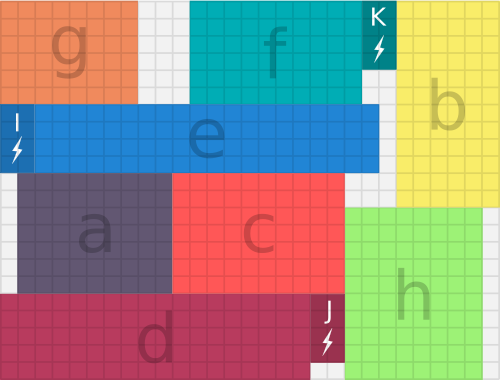
\includegraphics[scale=0.7]{power-grid-3.png}
		\caption{Placement of components on chip.}
	\end{figure}
	
	\section*{Problem 3: Ordering jobs}
	Satisfying all constraints, find a solution of this scheduling problem for which the total running time is minimal.


	\subsection*{Solution:}
	We generalize this problem to $n$ jobs. We have one variable {\tt running\_time} that we want to minimize and also for each job we introduce three variables, one for the start time, one for the end time and one for the duration of the job. So in total we introduce $3*n + 1$ variables. $ji\_s$ for $i = 1,\ldots,n$, denotes the start time of job $i$. $ji\_e$ for $i = 1,\ldots,n$, denotes the end time of job $i$. $ji\_d$ for $i = 1,\ldots,n$, denotes the duration of job $i$.
	
	As the jobs cannot start before a time of 0, we can express this by the formula
\[ \bigwedge_{i=1}^n (ji\_s \geq 0).\]

	Similarly, jobs cannot end after the total running time, which can be expressed by the formula
\[ \bigwedge_{i=1}^n (ji\_e \leq {\tt running\_time}).\]

	Next, we consider the duration of each job, which is given and can be expressed by the formula
\[ \bigwedge_{i=1}^n (ji\_d = i).\]

	As the jobs run without interruption, need to express that the end time of each job is equal to the start time plus the duration of that job. This can be expressed by the formula
\[ \bigwedge_{i=1}^n (ji\_e = (ji\_s + ji\_d)).\]

	Some jobs may not start before others have finished, so for each job $k \in K_i$, where $K_i$ is the set of jobs that need to be finished before job $i$ can start, we introduce a formula
\[ ji\_s \geq jk\_e.\]

	Finally, we also have some jobs that cannot run at the same time. So for every two distinct jobs $i,k \in D$, where $D$ is the set of jobs that are not allowed to run at the same time, either job $i$ needs to end before job $k$ can start, or job $k$ needs to end before job $i$ can start. For every two distinct jobs $i,k \in D$ this can be expressed with the formula
\[ (ji\_e \leq jk\_s) \vee (ji\_s \geq jk\_e).\]
	
For getting the answer to the minimization problem, we just try different values for the value of the variable {\tt running\_time} and see if we get a solution. When we find a solution for a value $x$ for {\tt running\_time} and we cannot find a solution for value $x-1$, we know that $x$ is the minimum amount of time we need to execute all the jobs.\\

After trying several values, we found that 36 is the minimal value for the running time of the jobs, since the program does not yield a solution for a running time of 35.\\

The total formula now consists of the conjunction of all these ingredients, that is,
\[ \bigwedge_{i=1}^n (ji\_s \geq 0) \;\; \wedge \]
\[ \bigwedge_{i=1}^n (ji\_e \leq {\tt running\_time}) \;\; \wedge \]
\[ \bigwedge_{i=1}^n (ji\_d = i) \;\; \wedge \]
\[ \bigwedge_{i=1}^n (ji\_e = (ji\_s + ji\_d)) \;\; \wedge \]
\[ \bigwedge_{k \in K_i} (ji\_s \geq jk\_e) \;\; \wedge \]
\[ \bigwedge_{i,k \in D; i \neq k} (ji\_e \leq jk\_s) \vee (ji\_s \geq jk\_e) \]


This formula is easily expressed in SMT syntax, for instance, for $n=12$ one can generate

{\footnotesize

{\tt (benchmark Assignment3.smt}

{\tt :logic QF\_LIA}

{\tt :extrafuns (}

{\tt ;Total running time }

{\tt (running\_time Int) }

{\tt ;Jobs, each with a duration, a start and an end }

{\tt (j1\_d Int) (j1\_s Int) (j1\_e Int) }
 
{\tt (j2\_d Int) (j2\_s Int) (j2\_e Int) }
 
$\cdots \cdots$
 
{\tt (j12\_d Int) (j12\_s Int) (j12\_e Int) }

{\tt )}

{\tt :formula}

{\tt   (and}

{\tt (>= j1\_s 0) (>= j2\_s 0) $\cdots$ (>= j12\_s 0) }

{\tt (<= j1\_e running\_time) }

{\tt (<= j2\_e running\_time) }

$\cdots \cdots$

{\tt (<= j12\_e running\_time) }

$\cdots \cdots$

{\tt )) }
}

Applying {\tt yices -m -smt Assignment3.smt} yields the following result
within a fraction of a second:

{\footnotesize

{\tt sat }

{\tt (= j7\_e 36) }

{\tt (= j12\_d 12) }

{\tt (= running\_time 36) }

{\tt (= j1\_e 7) }

{\tt (= j5\_d 5) }

{\tt (= j2\_s 5) }

{\tt (= j2\_d 2) }

{\tt (= j6\_e 29) }

{\tt (= j7\_d 7) }

{\tt (= j8\_s 7) }

{\tt (= j4\_e 10) }

$\cdots \cdots$ }

The start times of all the jobs are 

{\tt j1\_s = 6 }

{\tt j2\_s = 5 }

{\tt j3\_s = 7 }

{\tt j4\_s = 6 }

{\tt j5\_s = 10 }

{\tt j6\_s = 23 }

{\tt j7\_s = 29 }

{\tt j8\_s = 7 }

{\tt j9\_s = 15 }

{\tt j10\_s = 0 }

{\tt j11\_s = 13 }

{\tt j12\_s = 24 }

Expressed in a picture this yields

\begin{figure}[H]
	\centering
	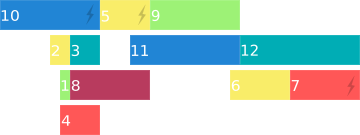
\includegraphics[scale=1]{timeline-2.png}
	\caption{Time-line of process execution.}
\end{figure}

\begin{figure}[H]
		\centering
			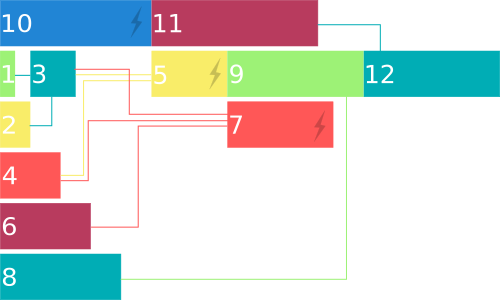
\includegraphics[scale=0.7]{timeline.png}
		\caption{A more organized solution to show that processes can be shifted. Connected and horizontal adjacent processes depend on each other, special processes are marked with a sign.}
\end{figure}

We check that indeed all requirements are satisfied and we also see that the total running time is 36, which is minimal.\\

{\bf Remark:}
Our variables contain some redundancy: the end time of each variable can already be derived from the start time and the duration of the job. We chose for this redundancy for keeping the symmetry in the solution, and also following the general strategy that introducing redundancy is often good for efficiency.\\

Note that with these constraints several different solutions are possible, since most of the smaller jobs can easily be shifted a bit in time.\\

{\bf Generalization:} 
As we generalized our approach for $n$ jobs rather than 12, it is interesting to see what happens for other values of $n$. For $n > 100$ we can still represent each job clearly, since we have no trouble with other integers that are near the job number. So if we keep the notation then it is still clear that {\tt j111\_s} represents the start time of job number 111.

\end{document}